\documentclass{article}
\usepackage[utf8]{inputenc}
\usepackage{amsmath,amssymb}
\usepackage{amsfonts}
\usepackage{paralist}
\usepackage{color}
\usepackage[table]{xcolor}
\usepackage{graphicx}
\usepackage{pgfplots}
\usepackage{authblk}
\usepackage{url}
\usepackage{multirow}
\usepackage{booktabs}
\usepackage{blindtext}
\usepackage{adjustbox}
\usepackage{subcaption}
\usepackage[margin=1.3in]{geometry}

\usepackage{float}
\usepackage[font=small, labelfont=bf, textfont=it, format=hang]{caption}
\usepackage[colorlinks=true, allcolors=blue]{hyperref}
\urlstyle{same}
\usepackage[english,nameinlink]{cleveref}
\usepackage{natbib} 
\crefname{equation}{}{}

\title{Cloud Computing Basic Final Project}
\author{Valentinis Alessio [SM3800008]}
\date{03/2024}

\begin{document}
	\maketitle
	\tableofcontents
	
	\section{Introduction}
	In this work, the aim was to assess the need of a Cloud File System, by using containarization through Docker and Docker-Compose, that enables users to seamlessly upload, download and deleting file and ensuring privacy of individual spaces, while enabling admins of some further operations and management of the structure, while not being able to access private space of the users. In order not to start everything from scratch I opted for using some pre-written utilities for Docker, by using Nextcloud image as frontend to manage the webUI.
	
	\section{What is Nextcloud and which features does it propose}
	For this work, I chose Nextcloud to adopt as a main application for managing my cloud deployement as it's an open-source solution which offers straight-away a lot of features, like user-friendly UI, robust and customizable security measures and the great scalability by its seamless association to Database Management Systems to manage the storing of the various data and metadata. Moreover the existance of a predefined Docker image makes this application a more than suitable choice, ensuring a simple lightweight deployement and a straightforward and fast usage.
	
	In this section I will be analyzing the features that make Nextcloud a secure and versatile environment to deploy a Cloud File System.
	
	\subsection{Nextcloud user authentication and authorization}
	
	Nextcloud offers straight-away built-in user authentication and authorization features that allow for different sign up and log in policies. In particular:
	\begin{itemize}
		\item \textbf{Registration and login}: Nextcloud offers a very simple registration and login processes out of the box, allowing each user to seamlessly sign up, log in or log out. Moreover, if an adim user isn't already created, the first user to sign to the service will be registered as admin: this may seem a huge problem, such as whoever comes first gets the privilege of being admin, but hopefully the provider will first set the whole service before making it available to the public.
	
		\item \textbf{Role-based access}: Nextcloud supports by default different users' roles, like simple users and admins. This policy ensures that each user is assigned the appropriate privileges, maintaining private user spaces.
		
		\item \textbf{Privare storage}: Nextcloud offers by default a private storage space to each user, by ensuring out-of-the-box isolation between different users. Furthermore, each user is allocated a predefined space, defined by a value in its configuration file: by defaults it ammounts to 512MB, but it's easilly modifiable by modifying a dotfile of the nextcloud container. This procedure will be further explained in the deployement section.
		
		\item \textbf{Admin capabilities}: Nextcloud offers admin a practical dashboard that allows him/her to easilly manage the entirety of the File System, by practically enabling encryption, security policies, add, limir and delete users, and much more.
	\end{itemize}
	
	By default, upon authentication, Nextcloud issues an access token that will be used for all future HTTP accesses, that will be stored only on the system of the client requesting it. On top of that, the password is stored encrypted in the associated Nextcloud database.
	
	By using Nextcloud out-of-the box, it doesn't allow for authonomous registration of the client, but only admins can generate its account. To enable this feature, it's necessary to install and enable the \verb|REGISTRATION| app, available on the \verb|User logo -> Applications| section of the admin dashboard: this way any new client can register to the system using the usual email-password credentials.
	
	\subsection{Security measures}
	Nextcloud comes with several out-of-the-box features regarding the security of the file system. In order to enamble the various security systems, the admin should simply go to the \verb|Administration| \verb|Settings -> Administration Security| and enable whichever module he wants. Some of them, however, require the installation of a dedicated app, available on the \verb|Application| page. One key feature that must be enabled when passing to production is SSE (Server Side Encryption), that enables the storage of users' data in an encrypted form, of course slowing down performance of the server and enlarging the size necessary to store a single file, but ensuring better security of the file system, above all in cases of sensible data. When SSE is enabled, a used is still capable of sharing files from the webUI, but he/she won't be able to share them from the server.
	To enable this feature, as specified above, you need to first download the \verb|Default Encryption| app, and then enable SSE from the \verb|Administration settings| page.
	
	Even taken these precautions, your system won't be secure unless you use very secure passwords. This constraint can be enable or modified from the same page of the \verb|Administration Settings|, by strengthening the passord policies. Other than this, to ensure even more secure access, we can enable two-factor authentication, always from the security section.
	
	% INSERT IMAGE OF THE ADMINISTRATION SETTINGS
	
	Of course, when passing from a private environment to a production framework, we can't rely on simple HTTP protocol to manage access to the service, forcing us to switch to HTTPS protocol to ensure better security and prevent attacks during communications.
	
	Furthermore, to secure even more the user-server communication and better load-balancing ratios, we can leverage a reverse proxy manager, like \textit{nginx} and connect the docker instance to an existing domain and managing SSL security policies.
		
	\subsection{Database solution and caching mechanism}
	
	To manage Nextcloud metadata, a default solution provided by the Nextcloud docker image with SQLite. In order to have a system that can be more similar to one that could be put in a production environment, I opted to implement a MariaDB database backend, which is supported straightawat from Nextcloud. Other than MariaDB, Nextcloud offers support also for PostgreSQL: at this point the choice of the Database differ only in performance and replication/backup systems, which are foundamental when we are talking about commercial suites to assess scalability and backup issues.
	
	Furthermore, to try and optimize performance, a caching mechanism has been provided through a Redis container. This solution aims to ease the response time and overall system workload by keeping a cahe of the recently analyzed files. Its benefits will be analyzed in the \ref*{sec:scalability} section.
	
	\subsection{Storage solutions}
	Nextcloud, if not instructed differently, stores all its files in the local file system, which may be a convenient choice if we limit ourselves to a small deployement. In more advanced environments it offers pretty straight-forward solution based on an existing Storage Server, also in the form of a distributed File System (NFS), or to an Object File System, like an Amazon S3 bucket. Based on the requirements, the optimal solution may vary and I'll discuss this topic in the \ref{sec:scalability} section.
	
	\subsection{Testing}
	In order to have a more convenient and well documented testing environment, with a pretty easy implementation and a practical monitoring tool, I opted to connect this environment to a \textit{Locust} instance, a well-known Python package that allows to simulate user interaction with the system at a customize workload rate. As a first approach I tried to manage this issue with a local instance of Locust, but I quickly realized on how many dependencies it counted on, making the use of a containerized instance of absolute importance. Furthermore, doing this I could practically access via web browser to its instance and monitor real-time the results of the test.
	
	\section{Deployement}
	The infrastructure has been deployed using Docker along with Docker Compose, which serves as a fundamental container orchestration tool developed by Docker. %Check this part.
	In particular, leveraging docker-compose orchestrating capabilities, we can deploy several docker containers and the respective network and volumes, only with one command: go to the main directory, containing the \verb|docker-compose.yml| file and perform
	
	\begin{verbatim}
		docker-compose up -d
	\end{verbatim}
	
	Doing this we have spawned:
	\begin{itemize}
		\item \textbf{Nextcloud} container with a dedicated volume
		\item \textbf{MariaDB} container with a dedicated volume
		\item \textbf{Locust} container
		\item A common \textbf{network} that connect all the containers.
	\end{itemize}
	
	Also, by just modifing the \verb|docker-compose.yml| file you can easilly modify the backend database, the network of the containers, also with the possibility of connecting it to an existing one.
	
	\subsection{Nextcloud setting}
	Before beginning, if you want to modify the maximum space allocated to each user of Nextcloud, you should modify a .dotfile into the Nextcloud instance.
	
	In order to do this, you can enter the Nextcloud container, through
	\begin{verbatim}
		docker exec -it nextcloud /bin/bash
		apt update
		apt install vim
		vim .htaccess
	\end{verbatim}
	And then paste this section
	\begin{verbatim}
		php_value memory_limit 2G
		php_value upload_max_filesize 4G
		php_value post_max_size 4G
		php_value max_input_time 3600
		php_value max_execution_time 3600
	\end{verbatim}
	
	Now you can access the container instantiation through \verb|http://localhost:8080|, and using the admin credentials set in the environment of the instance in the \verb|docker-compose.yml|, you can access in your admin account.
	Now your file system is up and running.
	
	\subsection{Testing with Locust}
	As previously announced, in order to assess the performance of my file system, I decided to use the Python library Locust.
	
	Before starting, it's useful to know that as a security measure, docker by default authorizes requests made only by the localhost. So, to le the locust container make all the requests, we have to add it to the \verb|trusted_domains| of the container. In order to achieve this result, we have to do this command:
	\begin{verbatim}
		docker exec --user www-data nextcloud /var/www/html/occ config:system:set
	\end{verbatim}
	\begin{verbatim}
		trusted_domains 1 --value=nextcloud
	\end{verbatim}
	
	\textbf{Warning}: If you don't perform this step, even if you are able to create all the users, tests launched from Locust will incur in \verb|permission denied| failure, failing all the tests.
	
	Once you have done this step, you can add all the users for the test, by simply perform the predefined script:
	\begin{verbatim}
		sh setup.sh
	\end{verbatim}
		
	Now, you should be up and running to perform your tests by logging to the Locust container through \verb|http://localhost:8089| and start swarming requests.
	
	To perform the test, I provided a \verb|locustest.py| that does different requests:
	\begin{itemize}
		\item PROPFIND: HTTP request that asks to retreive some metadata associated to a directory;
		\item GET: HTTP method that allows to retreive a default file created for each user;
		\item PUT: HTTP method that allows to put on the system a file. I developed 
		different methods that allows to upload (and right after delete, in order to preserve space) files of different sizes, namely 1kB, 1MB, 1GB in order to assess scalability of the system.
	\end{itemize}

	\textbf{Warning}: In the repository I didn't put the 1GB file, as it exceedes the maximum size allowed from GitHub. To create it, just
	\begin{verbatim}
		dd if=/dev/zero of=test_1gb bs=1M count=1024
	\end{verbatim}
	
	\subsection{Results of the load test}
	The test of the file system was conducted on my own PC, an Asus Vivobook15, with an Intel i7 10th gen CPU and 8GB of RAM, launching the containers from WSL on Windows. For all these tests, Server Side Encryption is enabled, so we expect in general worse performance.
	
	The test is divided in two parts, one concerning management of files up to 1MB, so sticking to a medium-size file, while the second part assess the management also of 1GB files.
	
	\begin{figure}[h]
		\centering
		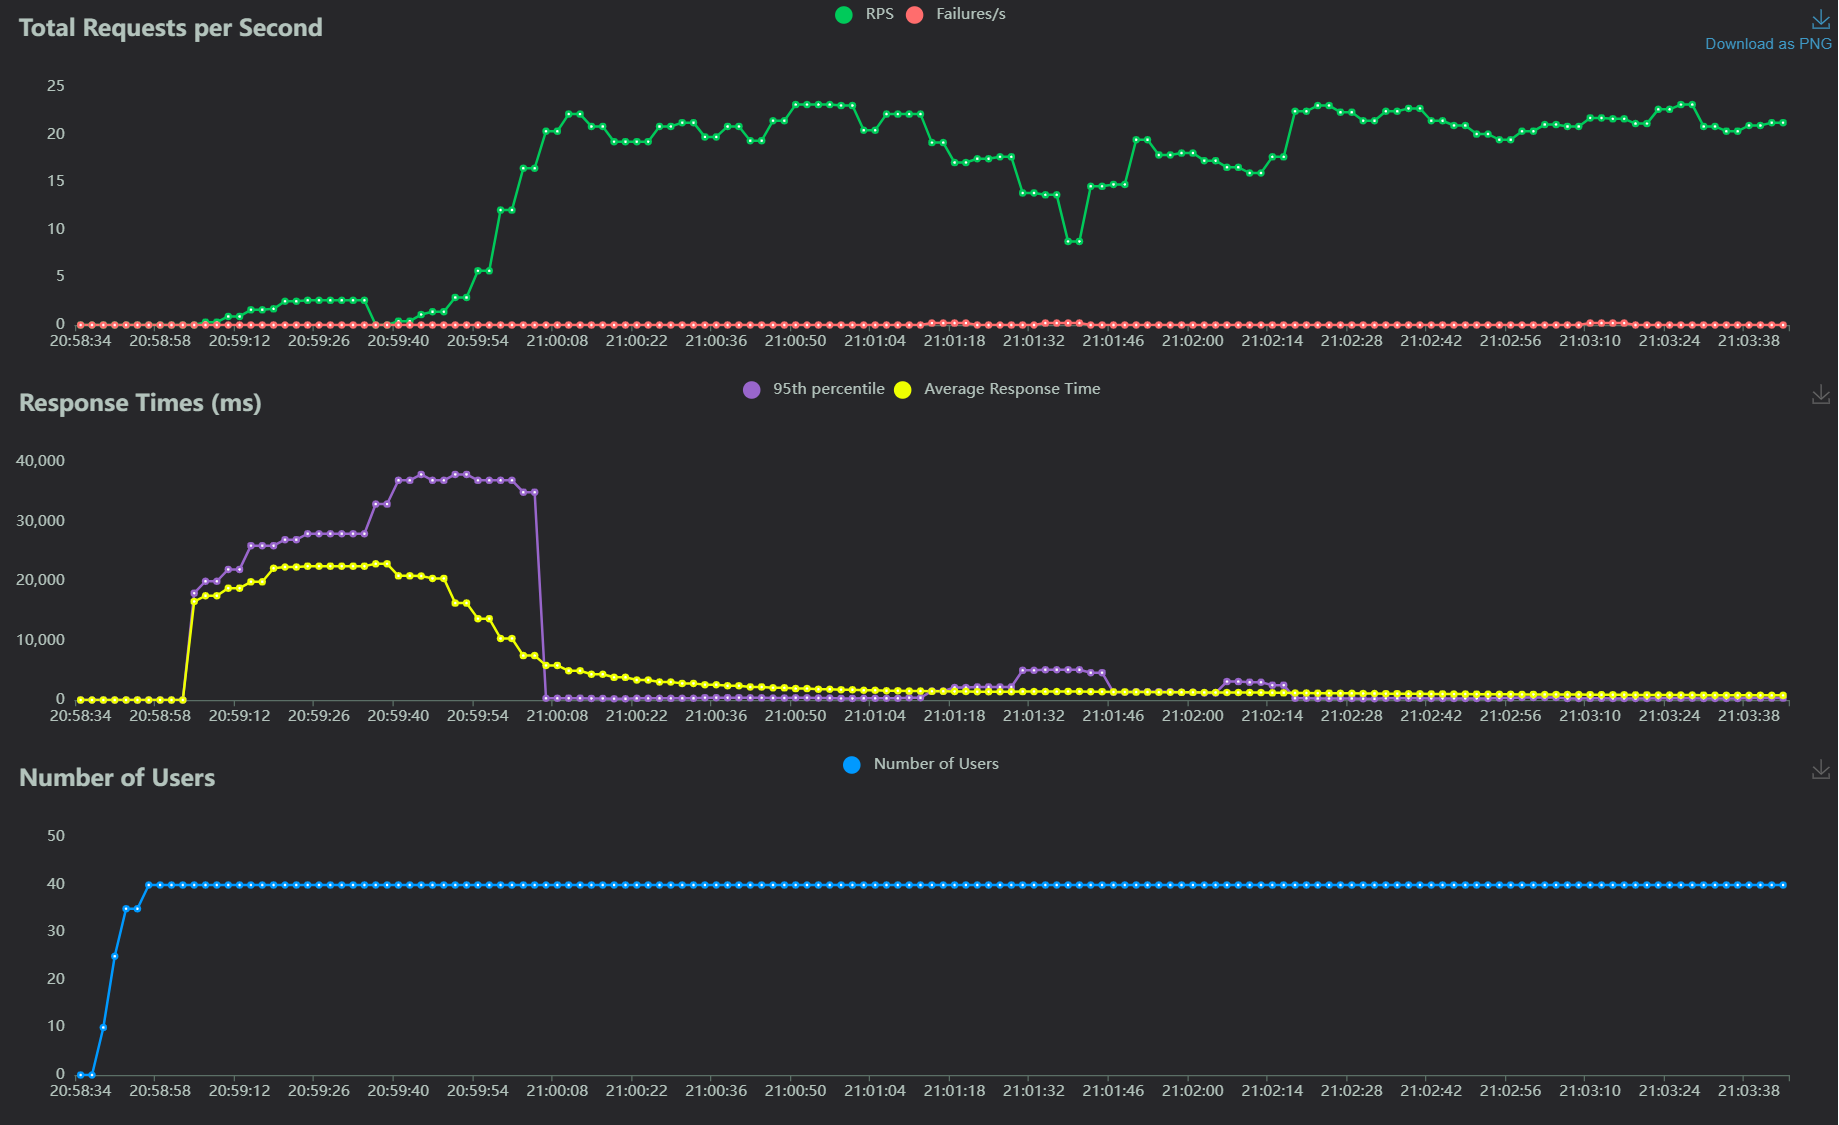
\includegraphics[width=0.7\linewidth]{total_requests_per_second_40user1mb}
		\caption{Load test for medium-sized files, 40 users.}
		\label{fig:totalrequestspersecond40user1mb}
		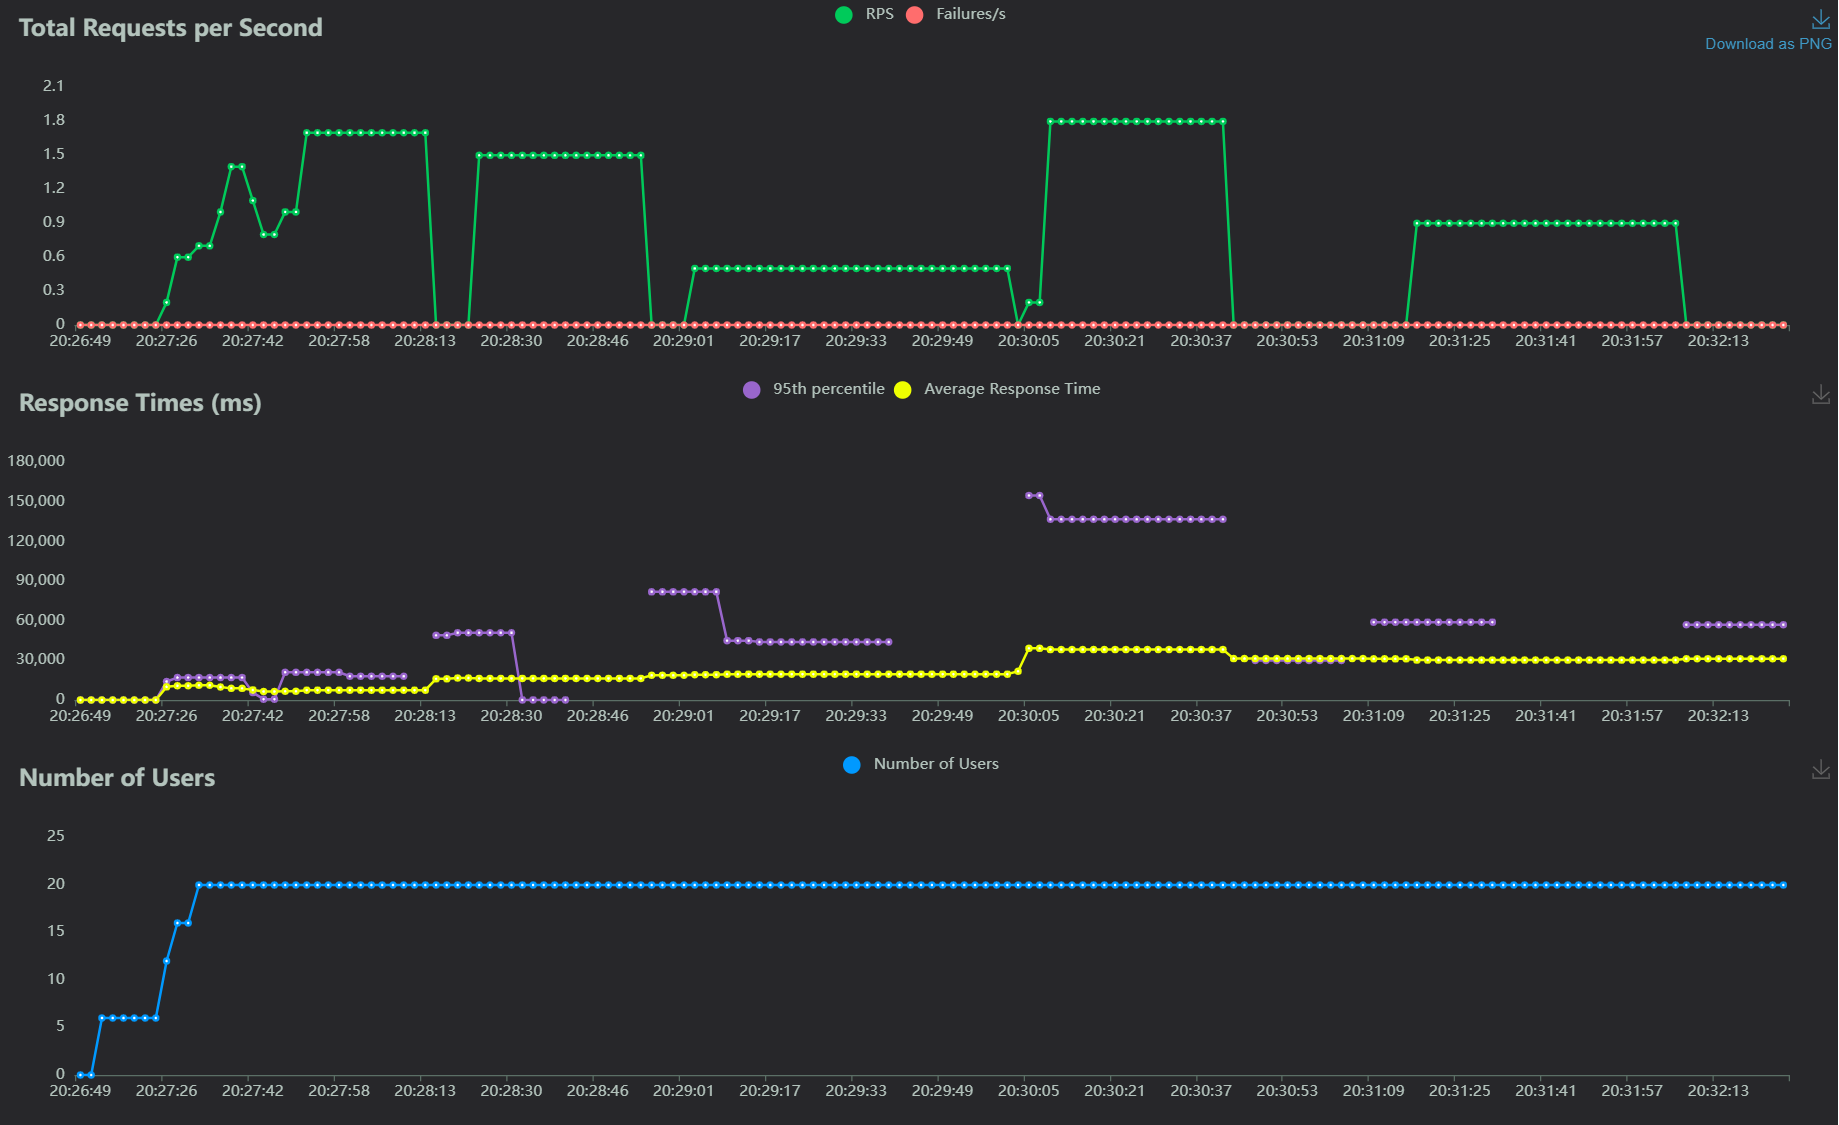
\includegraphics[width=0.7\linewidth]{response_times_(ms)_20users_1gb}
		\caption{Load test for large size files, 20 users.}
		\label{fig:responsetimesms20users1gb}
	\end{figure}
	
	As we can see from the figures \ref{fig:totalrequestspersecond40user1mb} and \ref{fig:responsetimesms20users1gb}, as long as we stick to medium-sized files, we have pretty good performance, being able to manage 40 users without any difficulty and satisfying more than 20 requests per second. Also the mean response time is fairly low, dropping below 1 second.
	
	Anyway, as soon as we switch to a large-sized file test, we are no more able to manage efficiently all the requests, stopping at less than 2 requests per second, with and average response time of about 30s. This fact of course should request more accurate tests, in order to pinpoint the exact problem, i.e. if we are delaing with an archietecture problem or an implementation problem. However, I'm pretty confident this is an archietecture issue, as the server doen't face any overload issue, as the number of failures sticks to zero: this give me confidence that the worse performance is most probably due only to an archietecture constraint, also consifìdering I'm managing these containers from WSL on a Windows machine (which by themselves occupy a lot of resources), and as soon as a 1GB PUT request is issued, the whole hardware is stuck to manage that request, so every other request is put on hold.
	
	\section{Scalability}
	\label{sec:scalability}
	In this section the aim is to propose some solutions to address an inreasing number of users and request for the delpoyed system, trying and analyze pros and cost issues of each.
	
	\subsection{Deployement on an existing NFS / Storage Server}
	If we suppose that a company already owns a storage Server, centralized or distributed, it should be optimal to deploy the Nextcloud instance with a shared ready database. In this context, a DBSM like PostgreSQL or MariaDB could be a suitable choice, as they are robust softwares, capable of managing many concurrent accesses, also from multiple nodes. To manage work balance between the different nodes, inplementing also a reverse-proxy instance, like said in the first section, may easilly ease the workload balance. Moreover, a backup and redundant system to ensure data availability and recovery in case of any kind of fail: for this purpose CEPH could be a suitable choice.
	
	\subsubsection{Advantages}
	\begin{itemize}
		\item \textbf{Infrastructure control}:  as we are delaing with a physical storage installation, the organization has full control over the infrastructure, making it easy to control.
		\item \textbf{Personalization}: dealing with a physical hardware upon which we are deploying a Nextcloud instance, can allow us to personalize the hardware infrastructure at need, based on required performance or compatibiliy with other hardwares.
		\item \textbf{Costs}: Being able to choose almost everything regarding the hardware on which we plan to base our deployement, besides the initial cost to deal with the actual hardware installation, all future costs of maintainability is much lower.
		\item \textbf{Security}: the organization can authonomously choose and implement its own security policy, without relying on other providers.
		\item \textbf{Location of data}: this solution ensures that the data stays into the physical or virtual infrastructure chosen by the organization, which is crucial when dealing with sensible data.
	\end{itemize}
	
	\subsection{Cloud Deployement}
	Opting for a Cloud provider may offer by default scalability and flexibility for your file system. One of the solution that can be assessed is relying on a cloud database, leveraging the horizontal scaling capability of the cloud provider to balance the load of the infrastructure.
	Data is considered to be stored in an Object File System, like Amazon S3, ensuring almost flawless scalability and storage capabilities. In order to satisfy variable workloads and manage accordingly the cost of the deployement, relying on the autoscalability feature of a cloud provider becomes a must.
	
	The choice of Amazon S3 as storage system comes from the capabilities of AWS services. Amazon Web Services offer robust autoscaling features, allowing for dynamical adjustment of the resources based on the demand of the infrastructure. Furthermore the principle of composability of its Object File System allows for seamless scaling of only those resources needed. Lastly, being based on an Object Storage System, it's suitable for handling large sized files, easilly offering also backup and replication options, and offering database systems, which can be used as backend for Nextcloud.
	
	\subsubsection{Advantages}
	\begin{itemize}
		\item \textbf{Scalability}: In general, cloud providers offer seamless horizontal scalability, allowing to quickly adapt on user demands and varying workload.
		\item \textbf{Managed services}: using a cloud provider can ease the need of infrastructure and database management, as offered by the provider.
		\item \textbf{World Wide Availability}: leveraging a cloud provider service, we implicitely rely on world-spread data centers, that enable global accessibility while ensuring consistent availability at reduced latency based on the region from which you are accessing the data.
		\item \textbf{Cost efficiency}: Leveraging the cloud, costs are based on the pay-as-you-go model, that can ease the costs for organizations with very variable workload demands.
	\end{itemize}
	
	\subsection{Cost efficiency assessment}
	Given these two possible solutions, what results to be the best way to go? Of course this has not a unique answer, and it highly depends on what are the needs of the organization that aims to use this service.
	
	If we are dealing with a pre-built hardware, in which we have a pre built infrastructure, like a cluster or a storage server, the first solution looks optimal, as we incur only in the first deployement and eventual infrastructure cost, but then operationally, the economic demand may actually be lower. This may be even more effective if a company has a "stable", or at least well known and almost constant workoad, or number of requests: of course this solution may incur in a higher initial economic loss, but then, if the archietecture is built optimized for the number and type of users that will access this service, this can rapidly overcome a cloud solution in terms of cost optimization, as future maintenance costs are most likely reduced to the minimum.
	
	Conversely to an industry or a company, which may already have a physical storage system or be already aware of the workload that would be necessary to manage, a single user, or a little startup, may not have a physical hardware available, or more importantly may not want to address the huge initial costs of deployement. If this is the case, the most sensible approach may be the second, as a pay-as-you-go policy may be more suitable as it can reduce costs above all for those realities where you don't precisely know of how much space do you need and of how much workload your deployement will be facing.
	
	So, the optimal solution may be dependent on how your hardware availability and how variable your workloads are. Also, if you wat to optimize the costs of your deployement, given that the files you are uploading in the cloud system are not sensible, Server-Side-Encryption may be disabled to optimize space-management.
	
	\section{Conclusions}
	In conclusion, this report outlined the implementation and assessment of a Cloud File System using Nextcloud, Docker, and Docker Compose. Nextcloud was chosen for its robust features, user-friendly interface, and scalability options. The report delved into various aspects, including user authentication and authorization, security measures, database solutions, storage options, and scalability considerations.
	
	Deployment was carried out using Docker and Docker Compose, allowing for easy orchestration of containers. Nextcloud settings were configured, including adjustments to user storage quotas. Testing was conducted using Locust, a Python library for simulating user interactions, to evaluate system performance under different workloads.
	
	Results showed satisfactory performance for managing medium-sized files but highlighted challenges with large-sized files, indicating potential architectural limitations. Scalability options were discussed, including deployment on existing NFS/storage servers and cloud-based solutions like Amazon S3. The choice between these options depends on factors such as existing infrastructure, workload variability, and cost considerations.
	
	Ultimately, the report provides insights into building and assessing a Cloud File System, highlighting both strengths and areas for improvement in system performance and scalability.
	
	
	
\end{document}